%% 美赛模板:正文部分

\documentclass[12pt]{article}  % 官方要求字号不小于 12 号,此处选择 12 号字体
\usepackage{float}
\usepackage{graphicx}
\usepackage{caption}
\usepackage{subcaption}
% 本模板不需要填写年份,以当前电脑时间自动生成
% 请在以下的方括号中填写队伍控制号
\usepackage[2021054]{easymcm}  % 载入 EasyMCM 模板文件
\problem{C}  % 请在此处填写题号
\usepackage{mathptmx}  % 这是 Times 字体,中规中矩 
%\usepackage{mathpazo}  % 这是 COMAP 官方杂志采用的更好看的 Palatino 字体,可替代以上的 mathptmx 宏包

\title{An MCM Paper Made by Team 1234567}  % 标题

% 如需要修改题头(默认为 MCM/ICM),请使用以下命令(此处修改为 MCM)
%\renewcommand{\contest}{MCM}

% 文档开始
\begin{document}

% 此处填写摘要内容
\begin{abstract}
    Here is the abstract of your paper.

    Firstly, that is ...

    Secondly, that is ...

    Finally, that is ...

    % 美赛论文中无需注明关键字。若您一定要使用,
    % 请将以下两行的注释号 '%' 去除,以使其生效
    % \vspace{5pt}
    % \textbf{Keywords}: MATLAB, mathematics, LaTeX.

\end{abstract}

\maketitle  % 生成 Summary Sheet
\tableofcontents  % 生成目录


% 正文开始
\section{Introduction}
\subsection{Problem Background}
Here is the problem background ...

Two major problems are discussed in this paper, which are:
\begin{itemize}
    \item Doing the first thing.
    \item Doing the second thing.
\end{itemize}

\subsection{Literature Review}
A literatrue\cite{1} say something about this problem ...

\subsection{Our work}
We do such things ...

\begin{enumerate}[\bfseries 1.]
    \item We do ...
    \item We do ...
    \item We do ...
\end{enumerate}

\section{Preparation of the Models}
\subsection{Assumptions}

\subsection{Notations}
The primary notations used in this paper are listed in Table \ref{tb:notation}.
\begin{table}[!htbp]
\begin{center}
\caption{Notations}
\begin{tabular}{cl}
	\toprule
	\multicolumn{1}{m{3cm}}{\centering Symbol}
	&\multicolumn{1}{m{8cm}}{\centering Definition}\\
	\midrule
	$A$&the first one\\
	$b$&the second one\\
	$\alpha$ &the last one\\
	\bottomrule
\end{tabular}\label{tb:notation}
\end{center}
\end{table}

\section{The Models}
\subsection{The subjectivity and polarity of a customer's review}
We assumed that each word, in the customers' reviews, has 2 properties: \textbf{subjectivity} and \textbf{polarity}. Subjective $s_{word}$ describes in what degree the word is subjective, ranges from 0 to 1. The higher $s_{word}$ is, the more subjective a word is. Polarity $p_{word}$ describes how much the customer loves or hates the product when writing the word, ranges from -1 to 1. We then define the subjectivity and the polarity of a sentences $s_{sentence}$ and $p_{sentence}$, which is the average of all the words in a sentences. Assume the number of words in a sentence is $n$, then
\begin{equation*}
  \begin{aligned}
    s_{sentence} = \dfrac{\sum\limits_{n} s_{word}}{n}  \\
    p_{sentence} = \dfrac{\sum\limits_{n} p_{word}}{n} 
  \end{aligned}
\end{equation*}
Apparently, if a customer A used 1 sentence to praise a product, and customer B used 10 sentences to praise it, customer B loves it more. So we sum up all the subjectivity and polarity of the sentences in customer's review, to indicate how subjective the customer is, and in what degree the customer loves or hates the product.
\begin{equation*}
  \begin{aligned}
    s_{customer} = \sum s_{sentence} \\
    p_{customer} = \sum p_{sentence}
  \end{aligned}
\end{equation*}
To solve this problem, of course we need a word list to store the subjectivity and polarity of different words. Perhaps we need machine learning. But in solving this problem, we didn't reinvent wheels because the wheel we invented probably won't better than the wheels in open source communities. So we used \textbf{textblob} , a python module, to calculate the subjectivity and polarity of the customers.

\subsection{The relation between rating levels and customer reviews}

To find the relation between rating levels and customer reviews, first we need to convert customer reviews, which is text based information, to numeric numbers. As we said in the previous section, we calculated the subjectivity and polarity of each customer, according to their reviews. And we used the \textbf{Curve Fitting} app in \textbf{MATLAB}, trying to fit a curve.
We imported the subjectivity, polarity and star ratings data of all the 3 products separately into \textbf{MATLAB}, and plotted the data. Then we could see from the graph that the polarity seemed to be linearly dependent with star rating, and the polarity is not dependent with star rating.
Then we used Linear Method to fit the data. These following graphs shows the relation between polarity, subjectivity and star rating of the 3 different products.
\begin{figure}[H]
  \centering
  \begin{subfigure}{.5\textwidth}
    \centering
    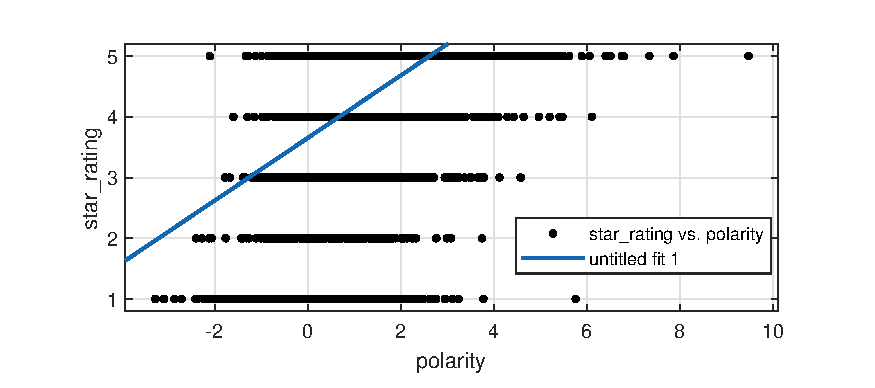
\includegraphics[width=\linewidth]{figures/hair_dryer/polarity_vs_star_rating.eps}
    \caption{star rating vs polarity}
    \label{fig:}
  \end{subfigure}%
  \begin{subfigure}{.5\textwidth}
    \centering
    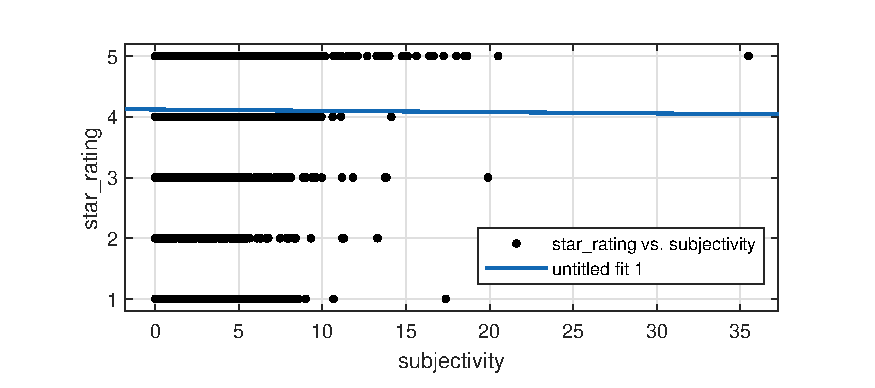
\includegraphics[width=\linewidth]{figures/hair_dryer/subjectivity_vs_star_rating.eps}
    \caption{star rating vs subjectivity}
    \label{fig:}
  \end{subfigure}
  \caption{the relation between polarity, subjectivity and star rating of the hair dryer}
  \label{fig:}
\end{figure}
\begin{figure}[H]
  \centering
  \begin{subfigure}{.5\textwidth}
    \centering
    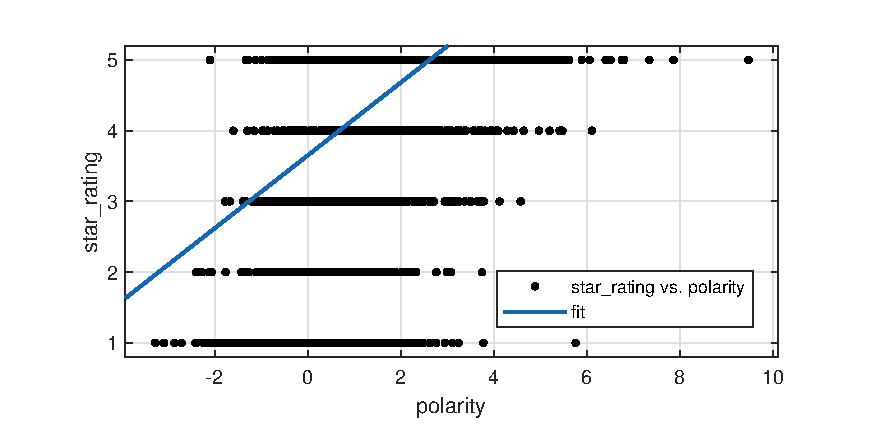
\includegraphics[width=\linewidth]{figures/microwave/polarity_vs_star_rating.eps}
    \caption{star rating vs polarity}
    \label{fig:}
  \end{subfigure}%
  \begin{subfigure}{.5\textwidth}
    \centering
    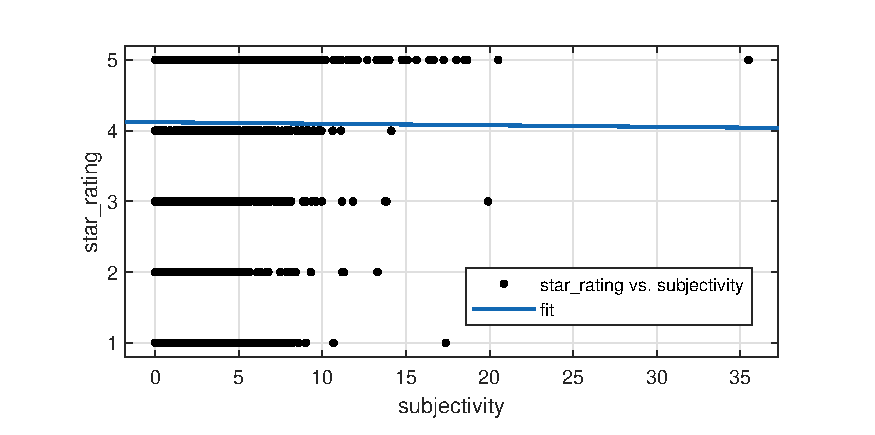
\includegraphics[width=\linewidth]{figures/microwave/subjectivity_vs_star_rating.eps}
    \caption{star rating vs subjectivity}
    \label{fig:}
  \end{subfigure}
  \caption{the relation between polarity, subjectivity and star rating of the microwave}
  \label{fig:}
\end{figure}
\begin{figure}[H]
  \centering
  \begin{subfigure}{.5\textwidth}
    \centering
    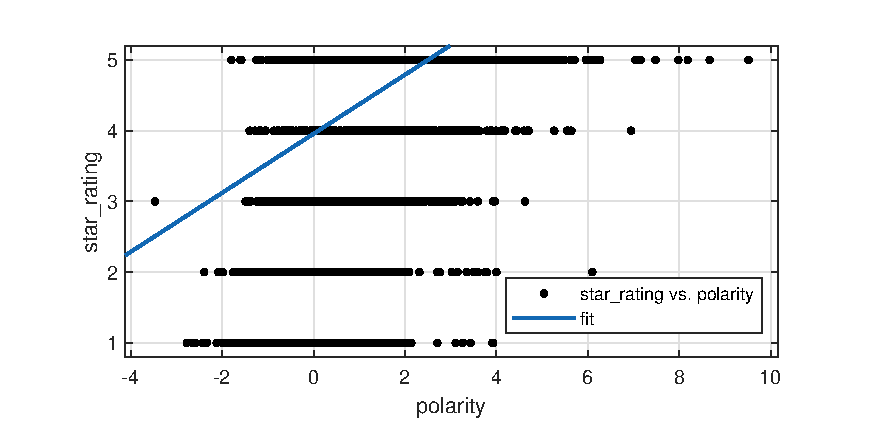
\includegraphics[width=\linewidth]{figures/pacifier/polarity_vs_star_rating.eps}
    \caption{star rating vs polarity}
    \label{fig:}
  \end{subfigure}%
  \begin{subfigure}{.5\textwidth}
    \centering
    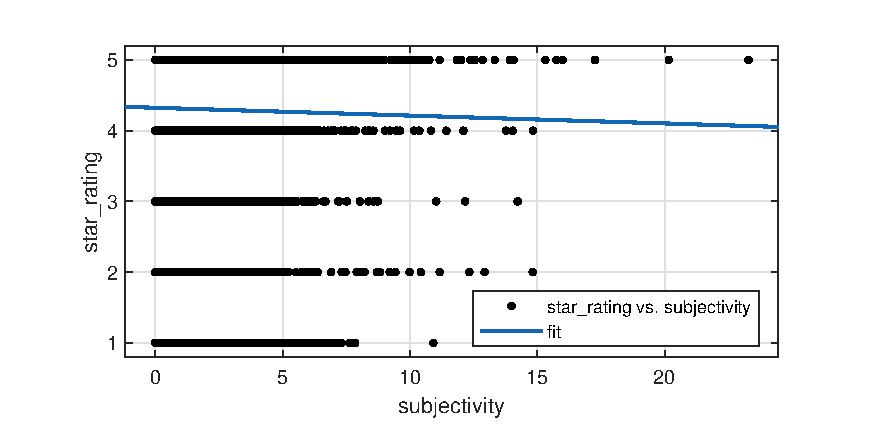
\includegraphics[width=\linewidth]{figures/pacifier/subjectivity_vs_star_rating.eps}
    \caption{star rating vs subjectivity}
    \label{fig:}
  \end{subfigure}
  \caption{the relation between polarity, subjectivity and star rating of the pacifier}
  \label{fig:}
\end{figure}
As \textbf{MATLAB} told us, the star rating, noted in $r$, is linearly related with customer's polarity $p$. And $r$ is unrelated with subjectivity of the customer $s$. For the hair dryer
\begin{equation*}
  \begin{aligned}
    r = 0.515 p + 3.652
  \end{aligned}
\end{equation*}
For the microwave
\begin{equation*}
  \begin{aligned}
    r = 0.5949 p + 2.969
  \end{aligned}
\end{equation*}
For the pacifier
\begin{equation*}
  \begin{aligned}
    r = 0.4172 p + 3.957
  \end{aligned}
\end{equation*}






\subsubsection{Detail 1 about Model 1}
The detail can be described by equation \eqref{eq:heat}:
\begin{equation}\label{eq:heat}
\frac{\partial u}{\partial t} - a^2 \left( \frac{\partial^2 u}{\partial x^2} + \frac{\partial^2 u}{\partial y^2} + \frac{\partial^2 u}{\partial z^2} \right) = f(x, y, z, t)
\end{equation}

\subsection{Model 2}
The results are shown in Figure \ref{fig:result}, where $t$ denotes the time in seconds, and $c$ refers to the concentration of water in the boiler.

\begin{figure}[htbp]
\centering
\includegraphics[width=.6\textwidth]{water.png}
\caption{The result of Model 2}\label{fig:result}
\end{figure}

\section{Strengths and Weaknesses}
\subsection{Strengths}
\begin{itemize}
    \item First one...
    \item Second one ...
\end{itemize}

\subsection{Weaknesses}
\begin{itemize}
    \item Only one ...
 \end{itemize}


% 以下为信件/备忘录部分,不需要可自行去掉
% 如有需要可将整个 letter 环境移动到文章开头或中间
% 请在后一个花括号内填写信件(Letter)或备忘录(Memorandum)标题
\begin{letter}{Memorandum}
\begin{flushleft}  % 左对齐环境,无首行缩进
\textbf{To:} Heishan Yan\\
\textbf{From:} Team XXXXXXX\\
\textbf{Date:} October 1st, 2019\\
\textbf{Subject:} A better choice than MS Word: \LaTeX
\end{flushleft}

In the memo, we want to introduce you an alternate typesetting program to the prevailing MS Word: \textbf{\LaTeX}. In fact, the history of \LaTeX\ is even longer than that of MS Word. In 1970s, the famous computer scientist Donald Knuth first came out with a typesetting program, which named \TeX\ \ldots

Firstly, \ldots

Secondly, \ldots

Lastly, \ldots

According to all those mentioned above, it is really worth to have a try on \LaTeX! 
\end{letter}


% 参考文献,此处以 MLA 引用格式为例
\begin{thebibliography}{99}
\bibitem{1} Einstein, A., Podolsky, B., \& Rosen, N. (1935). Can quantum-mechanical description of physical reality be considered complete?. \emph{Physical review}, 47(10), 777.
\bibitem{2} \emph{A simple, easy \LaTeX\ template for MCM/ICM: EasyMCM}. (2018). Retrieved December 1, 2019, from\url{https://www.cnblogs.com/xjtu-blacksmith/p/easymcm.html}
\end{thebibliography}


% 以下为附录内容
% 如您的论文中不需要附录,请自行删除
\begin{subappendices}  % 附录环境

\section{Appendix A: Further on \LaTeX}
To clarify the importance of using \LaTeX\ in MCM or ICM, several points need to be covered, which are \ldots

To be more specific, \ldots

All in all, \ldots

Anyway, nobody \textbf{really} needs such appendix \ldots

\end{subappendices}

\end{document}  % 结束